
% Camera-ready manuscript for EUMAS 2026 / Springer LNCS.
% Based on accepted submission, updated after reviewer comments and camera-ready instructions.
% Target venue: EUMAS 2026 / Springer LNCS.
\documentclass[runningheads]{llncs}

\usepackage[T1]{fontenc}
\usepackage{graphicx}
\usepackage{amsmath,amssymb}
\usepackage{booktabs}
\usepackage{array}
\usepackage{url}
\usepackage{xcolor}
\usepackage{hyperref}
\hypersetup{hidelinks}
\setlength{\textfloatsep}{6pt plus 1pt minus 2pt}
\setlength{\floatsep}{6pt plus 1pt minus 2pt}
\setlength{\intextsep}{6pt plus 1pt minus 2pt}
\setlength{\abovecaptionskip}{3pt}
\setlength{\belowcaptionskip}{0pt}
\emergencystretch=2em

\newcommand{\ind}{\mathbb{I}}
\newcommand{\clip}{\operatorname{clip}}
\newcommand{\argmaxop}{\operatorname*{arg\,max}}
\newcommand{\RR}{\textsc{Control}}
\newcommand{\IM}{\textsc{Integrated}}

\begin{document}

\title{Emotionally Bounded-Rational Agents in Repeated Games:\\
An Interpretable Dual-System Architecture and Diagnostic State-Stability Study}
\titlerunning{Emotionally Bounded-Rational Agents in Repeated Games}

\author{Dmitri Pavliuchenkov\inst{1}\thanks{Corresponding author.} \and Dmitri Gubanov\inst{2}}
\authorrunning{D. Pavliuchenkov and D. Gubanov}
\institute{Moscow Institute of Physics and Technology, Dolgoprudny, Russia\\
\email{pavliuchenkov.dm@phystech.edu}
\and
Institute for Control Sciences RAS, Moscow, Russia}

\maketitle

\begin{abstract}
Repeated social interaction is rarely reducible to material payoff alone: the same outcome can differ in fairness, relationship meaning, vulnerability, affective activation, and regulatory cost. We present an interpretable dual-system architecture for emotionally bounded-rational agents in repeated games. A game-to-values adapter maps external outcomes into material, fairness, relationship, and safety/no-regret event values; delta-based appraisal, mood, fatigue, and computational well-being then update the agent's internal state. A fast affective System~1 proposes action tendencies, while a slower System~2 can accept, override, or refocus them. We evaluate the implementation on 20 independent episodes of 200 rounds per condition in the Prisoner's Dilemma, Battle of the Sexes, and Ultimatum Game. The experiments compare a diagnostic-control mode, where adapter/appraisal quantities are logged for audit, with an integrated mode, where they participate in state updates. Under the specified internal-state aggregation, the integrated mode yields higher state scores and lower negative-state share across the tested scenarios, while still exposing exploitation, coordination failure, and game-specific stress-test artifacts. The paper should be read as a reproducible diagnostic architecture study rather than as a claim of human-behavioral or psychometric validation, or as a claim of strategic-performance superiority. The study is also positioned as the first reproducible layer of a broader programme: it defines the ablations, sensitivity checks, stronger baselines, and observer-validation steps needed to validate the proposed internal-state interpretation.
\keywords{Bounded rationality \and Emotional regulation \and Multi-agent simulation \and Repeated games \and Game-to-values adapter \and Internal-state diagnostics}
\end{abstract}

\section{Introduction}
Classical agent-based models and reinforcement-learning systems often represent strategic choice as the maximization of a single payoff or reward. This abstraction is useful for formal analysis, but it is too narrow for simulating repeated social interaction. In such settings, agents evaluate not only what they obtained, but also whether the outcome was fair, whether the partner supported or exploited them, whether cooperation made them vulnerable, and how costly it is to regulate emotional responses over time.

This paper addresses the problem of over-rationalized agents in repeated games. We do not merely add an ``emotion variable'' to a payoff optimizer. Instead, we separate the external game outcome from its subjective interpretation by the agent. A joint action first produces payoff and an outcome in the external environment. The outcome is then interpreted as a vector of internal event values: material payoff, fairness, relationship quality, and safety/no-regret. Changes in these values drive appraisal, mood, fatigue, and computational well-being, which in turn affect subsequent decisions.

The architecture is inspired by bounded rationality~\cite{simon1955behavioral}, dual-process decision-making~\cite{kahneman2011thinking}, prospect theory~\cite{kahneman1979prospect}, affective computing~\cite{picard1997affective}, appraisal theories of emotion~\cite{ortony1988cognitive,marsella2009ema}, and reinforcement learning~\cite{sutton2018reinforcement,mnih2015human}. Repeated games are used as compact diagnostic testbeds because they make payoff, fairness, coordination, exploitation, and adaptation observable under controlled conditions. We therefore use game theory as a controlled modeling language for social-interaction mechanisms, not as a claim that all emotion-related phenomena reduce to equilibrium analysis.

The study uses an architecture-aligned implementation in which game outcomes are processed through a value adapter and delta-based appraisal before they update mood, fatigue, well-being, and overall state. To make the methodological boundary explicit, the experiments include two model modes. The diagnostic-control mode is an audit and regression line: adapter/appraisal variables are reconstructed for explanation. The integrated-model mode is the main experimental setting: adapter/appraisal quantities participate in the state-update loop and can affect later decisions. This comparison is not an external calibration test. It is an internal state-stability and diagnostic-consistency test under a specified, auditable state score. More broadly, the paper is intended as a self-contained first layer of a longer research programme: it establishes the computational loop and reproducible evidence base on which white-box traces, ablations, stronger baselines, and observer validation can be built.

We make three methodological commitments. First, optimistic, neutral, and pessimistic denote parameter settings of the affective update rules; they should not be read as empirically validated personality categories. Second, the reported runs are diagnostic rather than confirmatory: they inspect mechanisms and failure modes, not statistical superiority. Third, the architecture does not eliminate scalarization. It relocates scalarization from raw payoff to a transparent internal-state score after value interpretation and affective-state updating. Accordingly, we do not claim that the model has been behaviorally or psychometrically validated against human data. Nor do we claim converged deep-RL policies or state-of-the-art MARL performance.

We organize the paper around four research questions:
\begin{itemize}
\item RQ1: Can a shared value-based affective-rational specification produce interpretable diagnostics across several repeated games without changing the overall architecture?
\item RQ2: How do hybrid, rational, emotional, and fixed-strategy agents differ in normalized payoff, game-specific metrics, and internal-state stability?
\item RQ3: Is there descriptive evidence of within-episode first-vs-last-third behavioral shifts under fixed partners?
\item RQ4: Which mechanisms and parameter choices contribute to state degradation, negative-state regimes, or recoverable failure modes?
\end{itemize}

The contributions are threefold: (i) an implementation-aware specification of an emotionally bounded-rational agent loop; (ii) a game-to-values adapter and state-update mechanism that make payoff--state divergence inspectable; and (iii) a reproducible diagnostic experiment package with validation checks, normalized per-game metrics, and explicit limits on interpretation. These contributions are complete for the present paper, while also defining the next layer of the project: white-box traces, ablations, stronger baselines, and validation of adapter and state interpretations.

\section{Related Work}
The work is positioned at the intersection of three research directions. The first is bounded rationality and social decision-making in games. Simon's bounded rationality~\cite{simon1955behavioral}, Kahneman's fast/slow distinction~\cite{kahneman2011thinking}, prospect theory~\cite{kahneman1979prospect}, and behavioral game theory~\cite{camerer2003behavioral} motivate models in which salience, loss, affect, and context shape decisions instead of a single ideal utility calculation. Game-theoretic baselines remain essential: Nash equilibrium~\cite{nash1950equilibrium}, Axelrod's analysis of cooperation and tit-for-tat~\cite{axelrod1984evolution}, and behavioral models of fairness, inequity aversion, guilt, and punishment~\cite{guth1982ultimatum,bolton2000erc,charness2002understanding,fehr1999theory,rabin1993fairness,battigalli2007guilt,battigalli2022belief,fehr2002punishment} frame our use of repeated games and internal value dimensions. The behavioral-economics role of these references is conceptual: they justify modeling subjective interpretation, social comparison, and regret-sensitive evaluation, while the present experiments remain computational diagnostics rather than behavioral estimates from human-subject data.

The second direction is affective agent architecture. Existing systems include OCC-style appraisal~\cite{ortony1988cognitive}, EMA~\cite{marsella2009ema}, ALMA~\cite{gebhard2005alma}, WASABI~\cite{beckerasano2010wasabi}, FAtiMA~\cite{dias2014fatima}, and MAMID~\cite{hudlicka2004mamid}; emotion in reinforcement learning has also been surveyed in robotics and RL~\cite{moerland2018emotion}. Risk-as-feelings and computational work on emotion in strategic interaction further motivate affective state as more than a reward-shaping trick~\cite{loewenstein2001risk}. Our contribution is narrower than a complete cognitive architecture: we build a compact repeated-game prototype in which value interpretation, mood, fatigue, well-being, and appraisal diagnostics are explicit and inspectable.

The third direction is multi-agent learning in social dilemmas. Modern MARL emphasizes non-stationarity, cooperation, communication, contracts, and evaluation~\cite{gronauer2022marl,zhu2024communication,ning2024survey,mu2024socialdilemmas,haupt2024contracts,willis2024reward,su2026iterated}. These works motivate caution: claims about repeated-game adaptation require longer horizons, multiple seeds, game-sensitive metrics, and strong baselines. The present work therefore does not compete with MARL benchmarks or social-preference utility models. It instead provides a transparent bridge from external game outcomes to auditable internal-state diagnostics.

\begin{figure}[t]
\centering
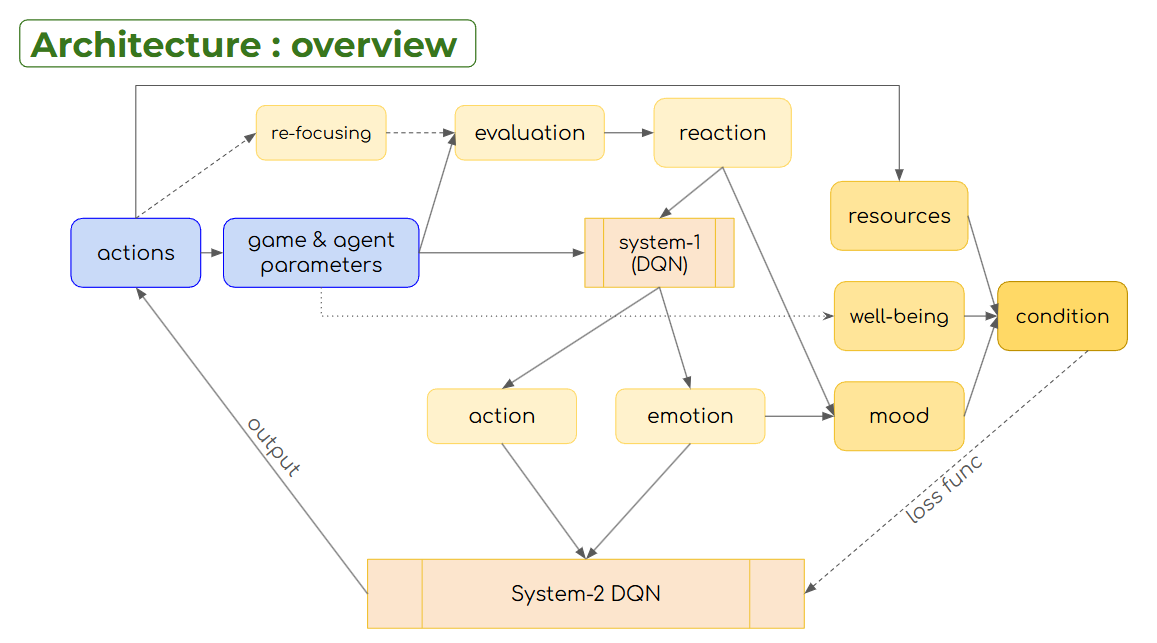
\includegraphics[width=.96\linewidth]{figures/architecture_v14.png}
\caption{Architecture overview. The diagram shows the implementation-level control loop: game and agent parameters feed re-focusing, evaluation, reaction, System~1 DQN, System~2 DQN, and the internal-state variables used by the agent. The formal adapter, state-update equations, and the diagnostic-control versus integrated modes are specified in Sections~\ref{sec:model}--\ref{sec:protocol}.}
\label{fig:architecture}
\end{figure}

\section{Model Specification}
\label{sec:model}
The model is a closed affective-cognitive loop: observe a repeated-game state, choose an action, receive an outcome and material payoff, interpret the outcome as event values, update internal values and affective state, and use the updated state in later decisions. Figure~\ref{fig:architecture} gives the implementation-level overview; the formal adapter, state update, and two experimental modes are defined below.

\subsection{External Game and Value Interpretation}
A repeated game is modeled as an external environment
\[
G=(N,S,A,T,R,\Omega),
\]
where $N$ is the set of agents, $S$ the game-state space, $A=(A_i)_{i\in N}$ the family of legal action sets, $T$ the transition/outcome rule, $R=(R_i)_{i\in N}$ the family of material payoff functions, and $\Omega$ the outcome space. At step $t$, agent $i$ chooses $a_{i,t}\in A_i$, the environment returns outcome $o_t\in\Omega$, and the material payoff is $\pi_{i,t}=R_i(o_t)$.

The game-to-values adapter separates the external result from its subjective meaning for a focal agent:
\[
\mathcal{A}^G_i(a_i,a_j,\pi_i,\pi_j)\mapsto q_i=(q^{mat}_i,q^{fair}_i,q^{rel}_i,q^{safe}_i)\in[0,1]^4.
\]
Table~\ref{tab:values} gives the proxies used in the implementation. The safety dimension is deliberately described as a safety/no-regret or ex-post vulnerability proxy: it measures how exposed the agent was to a worse-than-best response, not broad physical or social safety.

\begin{table}[t]
\centering
\caption{Subjective event values returned by the game-to-values adapter.}
\label{tab:values}
\scriptsize
\begin{tabular}{p{.20\linewidth}p{.24\linewidth}p{.31\linewidth}p{.17\linewidth}}
\toprule
Value & Meaning & Operational proxy & Role \\
\midrule
Material payoff & Agent's material outcome. & Payoff normalized by the feasible payoff range of the agent in the game. & Links to classical game payoffs. \\
Fairness & Perceived symmetry of the outcome. & $1-|\tilde\pi_i-\tilde\pi_j|$, using normalized payoffs. & Captures unfairness and bargaining sensitivity. \\
Relationship & Whether the partner supported or harmed the agent given the agent's action. & Actual payoff relative to best/worst payoff obtainable under the observed partner action. & Represents trust, betrayal, and repair. \\
Safety/no-regret & Protection from exploitation, operationalized as ex-post vulnerability. & $1-$ normalized regret relative to the best response to the partner's action. & Proxy for exposure to a worse-than-best response. \\
\bottomrule
\end{tabular}
\end{table}

Event values update accumulated internal values through exponential smoothing:
\[
v_{i,k}(t+1)=(1-\alpha_k)v_{i,k}(t)+\alpha_k q_{i,k}(t),\quad \alpha_k\in[0,1],
\]
with clipping to $[0,1]$ when required. This is a modeling choice: all target values are currently set to $v^*_{i,k}=1$, meaning that more material satisfaction, fairness, relationship quality, and no-regret safety is treated as better. Alternative targets and windowed updates are left to sensitivity analysis.

\subsection{Internal State, Appraisal, and Model Modes}
Each agent maintains an internal value state $v_i(t)\in[0,1]^4$, priorities $p_i$ with $\sum_{k\in K} p_{i,k}=1$, mood $m_i(t)$, fatigue $f_i(t)$, well-being proxy $w_i(t)$, and overall state score $S_i(t)$. Well-being is the weighted degree of value satisfaction:
\[
w_i(t)=\sum_k p_{i,k}v_{i,k}(t).
\]
The overall state score is an interpretable first-order aggregation:
\[
S_i(t)=\lambda_w w_i(t)+\lambda_m m_i(t)-\lambda_F f_i(t).
\]
In the reported runs, $\lambda_w=\lambda_m=\lambda_F=1$, so $S_i=w_i+m_i-f_i$. This score is a computational diagnostic, not a psychometric well-being scale.

For each value $k$, urgency measures the subjective criticality of a value change. If $\Delta v_{i,k}(t)=v_{i,k}(t)-v_{i,k}(t-1)$, then
\[
u_{i,k}(t)=
\begin{cases}
\min\left(1,\frac{|\Delta v_{i,k}(t)|}{\max(\epsilon,1-v_{i,k}(t-1))}\right), & \Delta v_{i,k}(t)>0,\\
\min\left(1,\frac{|\Delta v_{i,k}(t)|}{\max(\epsilon,v_{i,k}(t-1))}\right), & \Delta v_{i,k}(t)<0,\\
0, & \Delta v_{i,k}(t)=0.
\end{cases}
\]
Gains are normalized by remaining distance to the target, while losses are normalized by the already attained value. Signed urgency is $\operatorname{sgn}(\Delta v_{i,k})u_{i,k}$. Valence and emotional load are
\[
V_i(t)=\sum_k p_{i,k}\operatorname{sgn}(\Delta v_{i,k})u_{i,k},\qquad
L_i(t)=\sum_k p_{i,k}u_{i,k}.
\]
Valence captures direction; load captures intensity regardless of sign. Attention focus is $k^*_i(t)=\argmaxop_k p_{i,k}u_{i,k}$.

The reported implementation uses two modes. In diagnostic-control mode, adapter/appraisal variables are logged for audit and comparison. In integrated mode, they participate in value and affective-state updates. Table~\ref{tab:status} summarizes the distinction.

\begin{table}[t]
\centering
\caption{Status of major mechanisms in the current article.}
\label{tab:status}
\scriptsize
\begin{tabular}{p{.28\linewidth}p{.26\linewidth}p{.36\linewidth}}
\toprule
Component & Status & Role \\
\midrule
Learned two-system agents & Behavior-driving & Core policy mechanism for hybrid, emotional, and rational comparisons. \\
Mood, fatigue, well-being, overall state & Behavior-driving/logged & Implemented state variables and main internal-state diagnostics. \\
Adapter/appraisal in diagnostic-control mode & Diagnostic/explanatory & Reconstructed from logs for audit; not direct DQN inputs in this control mode. \\
Adapter/appraisal in integrated mode & Behavior-driving via state update & Event values and appraisal affect value and state updates and therefore later decisions. \\
Suppression-cost proxy & Diagnostic/planned & Logged or reconstructed to interpret regulation costs; a fully white-box suppression-cost update is future work. \\
\bottomrule
\end{tabular}
\end{table}

\subsection{Affective State Updates}
The implementation uses bounded state updates. A compact formal abstraction is
\[
e_i(t)=\clip(\eta_V V_i(t)+\eta_L L_i(t),-1.5,1.5),
\]
where $e_i(t)$ is valenced emotional intensity. Mood and fatigue are updated as
\[
m_i(t+1)=\clip(\rho_m m_i(t)+\kappa_m e_i(t),-0.5,0.5),
\]
\[
f_i(t+1)=\clip((1-\rho_f)f_i(t)+\rho_f(\beta L_i(t)+(1-\beta)|e_i(t)|),0,1).
\]
These equations implement the architecture-aligned mechanism used in the reported runs: value changes, not the mere distance from a target, drive mood and fatigue. Parameter values and code hashes are stored in the run manifests.

\section{Dual-System Control}
DQN denotes a Deep Q-Network: a value-based reinforcement-learning method that approximates action values with a neural network. In this paper, the term DQN-like refers to the trainable action-selection modules used inside the agent architecture, rather than to a claim of converged deep-RL performance. Each module receives a numeric state vector, selects an action or control option using an epsilon-greedy policy over learned Q-values, stores transitions in a replay buffer, and updates a neural network by minibatch Bellman-style targets with a slower target network:
\[
y_t=r_t+\gamma\max_{a'}Q(s_{t+1},a';\theta^-),\qquad
\mathcal{L}(\theta)=(y_t-Q(s_t,a_t;\theta))^2.
\]
The implementation uses two hidden ReLU layers with 128 units, Adam with learning rate $10^{-3}$, replay buffers up to 1000 transitions, minibatches up to 32, $\gamma=0.99$, epsilon decay $1.0\rightarrow0.01$ with factor $0.995$, target-network update period 1000, and 10 parameter bins. System~1 is trained on current-state-evaluation feedback; System~2 is trained on the overall-state objective or its change. The state vector includes game/action information, current internal state variables, and mode-dependent value/appraisal summaries; the exact serialized fields are documented in the artifact schema. Because each episode has 200 rounds, these modules are treated as short-horizon trainable prototype policies, not fully converged deep-RL solutions.

System~1 is the fast affective mechanism. In the learned implementation it proposes an action tendency with valenced intensity. System~2 is the slower control mechanism. It accepts, overrides, or refocuses the proposal and is trained to improve the overall internal-state score. An emotional impulse dominates if its intensity exceeds a fatigue-dependent threshold:
\[
\theta_i(t)=\clip(\theta_{0,i}(1-\lambda_\theta f_i(t)),\theta_{min},\theta_{max}),
\]
where $\lambda_\theta$ is distinct from the state-aggregation weight $\lambda_F$. Table~\ref{tab:pipeline} summarizes the one-step loop. The external game is executed once, outside the agent; the agent decides, observes the actual outcome, and then updates state.

\begin{table}[t]
\centering
\caption{Compact one-step decision/update pipeline.}
\label{tab:pipeline}
\scriptsize
\begin{tabular}{p{.07\linewidth}p{.84\linewidth}}
\toprule
Step & Operation \\
\midrule
1 & Observe game state, legal actions, previous value changes, mood, fatigue, and current internal state. \\
2 & System~1 proposes an affective action tendency and emotion intensity from the implemented state vector. \\
3 & Compare impulse intensity with the fatigue-dependent threshold; if it dominates, execute the emotional action. \\
4 & Otherwise System~2 accepts, overrides, or refocuses the proposal according to the overall-state objective. \\
5 & Execute joint actions in the external game and observe payoffs/outcome. \\
6 & Apply the adapter, update values, appraisal, mood, fatigue, well-being and overall state, then store training transitions and logs. \\
\bottomrule
\end{tabular}
\end{table}

\section{Experimental Protocol}
\label{sec:protocol}
The experiments use the paper profile: 20 independent episodes of 200 rounds per condition, fixed scenario definitions, strict error policy, no fallback rows, and automatically saved CSV/figure artifacts. One episode is a complete repeated interaction under a fixed game, agent pair, configuration, and seed; one round is a single stage-game interaction inside that episode. The seed set is fixed and stored in each manifest. Ordered pairs are kept distinct because role, payoff split, and agent-specific internal state can differ between, for example, Hybrid--Rational and Rational--Hybrid.

The games are the Prisoner's Dilemma (PD), Battle of the Sexes (BoS), and Ultimatum Game (UG). Table~\ref{tab:protocol} summarizes the game definitions and metrics. Payoff values are normalized by the feasible game-specific pair payoff when comparing across games: $1200$ for PD, $1000$ for BoS, and $2000$ for UG over 200 rounds. Raw payoffs are reported only within game-specific tables or as descriptive condition values.

\begin{table}[t]
\centering
\caption{Game definitions, paper-profile scale, and aggregation.}
\label{tab:protocol}
\scriptsize
\begin{tabular}{p{.20\linewidth}p{.70\linewidth}}
\toprule
Block & Setting \\
\midrule
Paper profile & S1--S4; 20 independent episodes; 200 rounds; strict validation; all reported values are descriptive means unless dispersion is shown. \\
Games & PD: $CC=(3,3)$, $CD=(0,5)$, $DC=(5,0)$, $DD=(1,1)$. BoS: $(O,O)=(3,2)$, $(F,F)=(2,3)$, mismatches $(0,0)$. UG: fixed proposer/responder roles, discretized offers, and accept/reject outcomes. \\
Metrics & PD: mutual cooperation and exploitation. BoS: agreement and coordination. UG: acceptance rate, mean offer, fair-offer rate. Internal metrics: overall state and negative-state share $\Pr(S_i<0)$. \\
Agents & Hybrid, emotional-only, rational-only, and fixed strategies. Fixed strategies are cleanest in PD; BoS/UG fixed rows are treated as stress tests unless game-specific semantics are explicit. \\
Statistics & Means over 20 episodes; selected tables include episode-level standard deviations where compact enough. No significance tests or superiority claims are made. \\
\bottomrule
\end{tabular}
\end{table}

The scenarios are: S1, an ordered cross-type matrix; S2, a fixed-partner first-vs-last-third trend proxy; S3, a profile/intensity sensitivity sweep; and S4, state-diagnostics cases. All official runs passed validation: no missing files, no fallback rows, no out-of-range mood/fatigue, no NaN/inf values, and no duplicate observe events.

\section{Results}
Reading guide: S1 evaluates cross-type comparisons, S2 gives a first-vs-last-third trend proxy, S3 is an affective-profile sensitivity check, and S4 analyzes state degradation. All claims are descriptive and diagnostic. The central empirical quantity is not raw payoff pooled across games, but normalized payoff together with game-specific social metrics and internal-state diagnostics.

\subsection{Two-Mode State-Stability Overview}
Table~\ref{tab:modeoverview} summarizes the two-mode comparison using normalized payoff, mean pair state, and negative-state share. The integrated model raises mean pair state and lowers negative-state share in all four scenarios under the specified internal-state aggregation. This is not external calibration and not proof of human-like behavior. It means that after adapter/appraisal variables become part of the state-update loop, the state score is less dominated by artificial negative saturation and more dependent on game/partner conditions.

\begin{table}[t]
\centering
\caption{Scenario-level overview. Normalized payoff divides pair payoff by each game's feasible 200-round maximum before averaging across games and conditions.}
\label{tab:modeoverview}
\scriptsize
\begin{tabular}{llrrrr}
\toprule
Scenario & Mode & Cond. & Norm. payoff & Pair state & Neg. share \\
\midrule
S1 & Integrated & 48 & 0.790 & 0.240 & 0.213 \\
S1 & Control & 48 & 0.755 & -0.154 & 0.471 \\
S2 & Integrated & 27 & 0.681 & 0.232 & 0.253 \\
S2 & Control & 27 & 0.666 & -0.225 & 0.541 \\
S3 & Integrated & 27 & 0.791 & 0.108 & 0.277 \\
S3 & Control & 27 & 0.780 & -0.044 & 0.328 \\
S4 & Integrated & 12 & 0.559 & 0.000 & 0.471 \\
S4 & Control & 12 & 0.519 & -0.364 & 0.612 \\
\bottomrule
\end{tabular}
\end{table}

\begin{figure}[t]
\centering
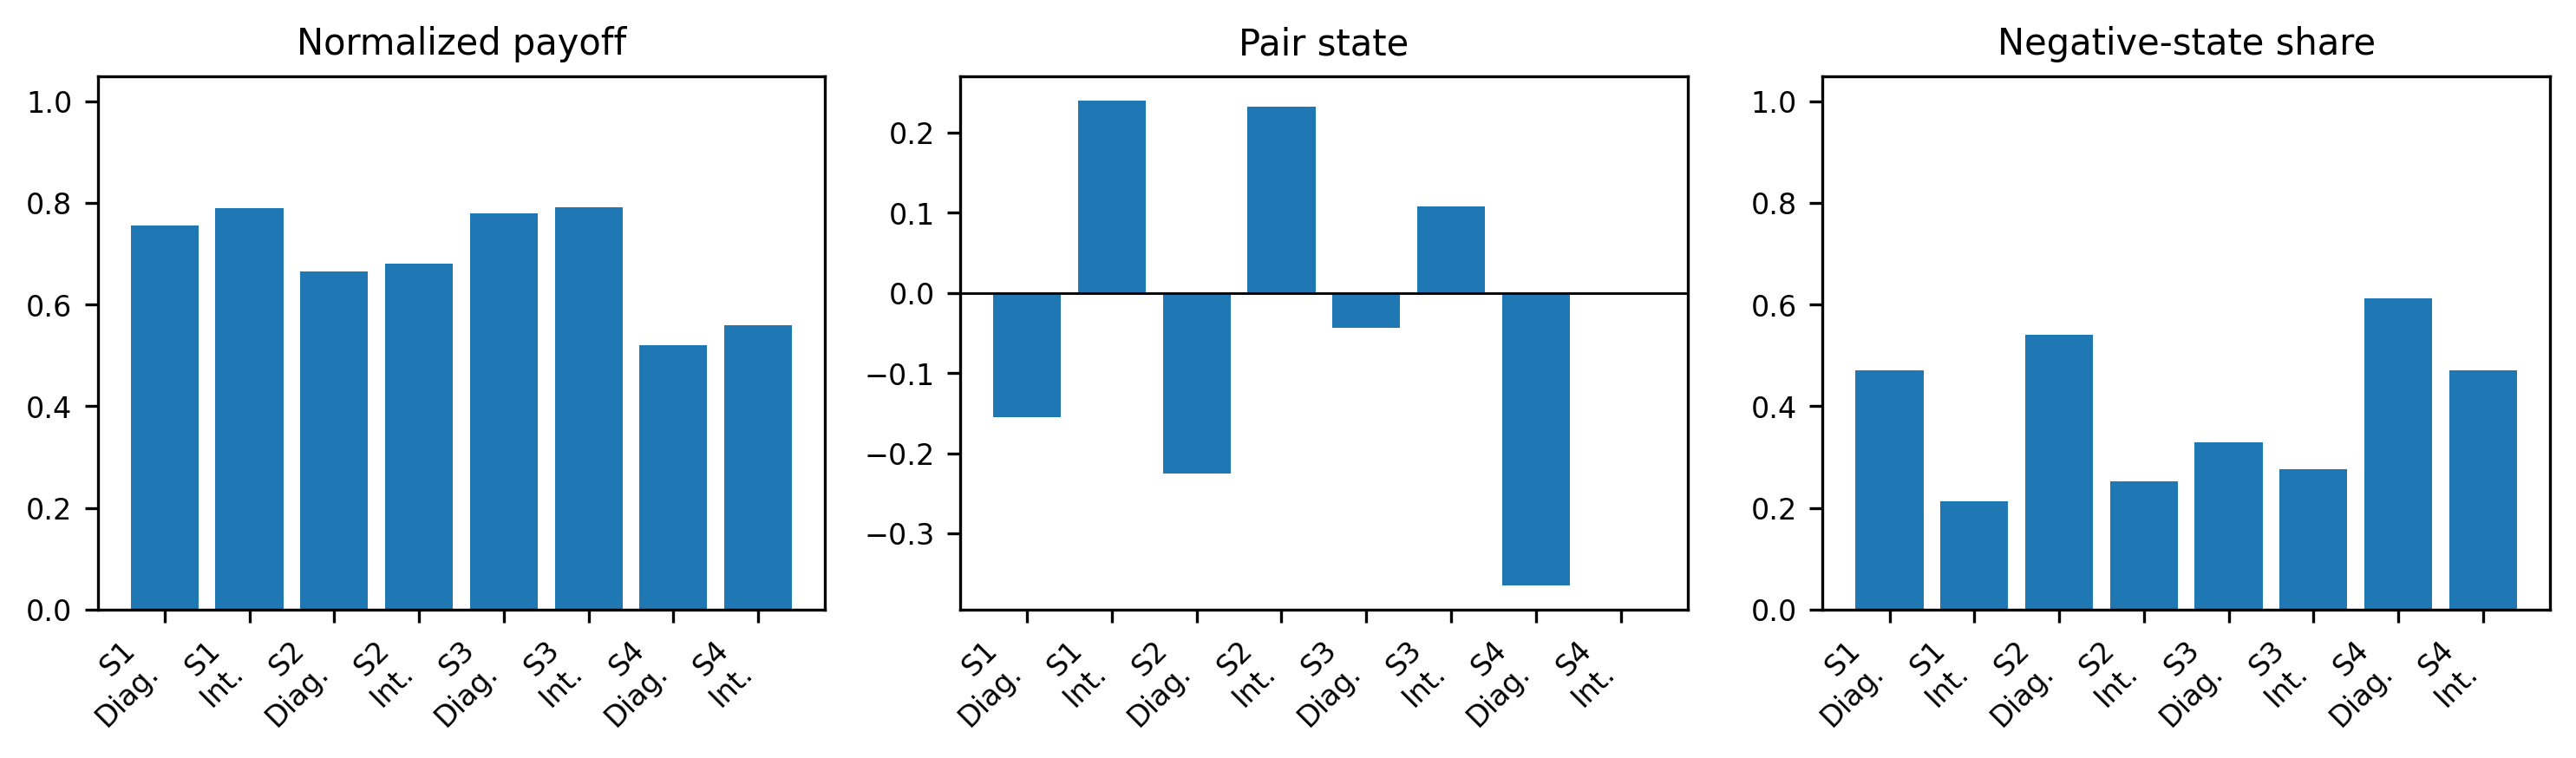
\includegraphics[width=.96\linewidth]{figures/fig_scenario_mode_overview_normalized.png}
\caption{Scenario-level comparison of diagnostic-control and integrated modes. Payoff is normalized within each game before aggregation.}
\label{fig:mode_overview}
\end{figure}

Figure~\ref{fig:mode_overview} visualizes the same pattern. Some improvements are large in state variables and modest in normalized payoff; this is expected because the intervention changes the state-update loop rather than optimizing raw payoff directly.

\subsection{S1: Cross-Type Matchups}
S1 contains 48 ordered conditions in each mode. Table~\ref{tab:s1} reports selected integrated-model conditions. The selection contrasts hybrid, rational, emotional, and fixed-strategy baselines across games; the full matrix is included in the artifact bundle. Normalized payoff and pair state are reported as mean $\pm$ standard deviation across episodes. Figure~\ref{fig:s1tradeoff} shows the payoff--state trade-off for these selected conditions.

\begin{table}[t]
\centering
\caption{Selected S1 integrated-model comparisons. Metric is mutual cooperation in PD, agreement in BoS, and acceptance rate/mean offer in UG.}
\label{tab:s1}
\scriptsize
\begin{tabular}{llccc}
\toprule
Game & Pair & Norm. payoff & Pair state & Metric \\
\midrule
PD & Hybrid vs Hybrid & 1.000 $\pm$ 0.000 & 0.281 $\pm$ 0.000 & 1.0 \\
PD & Hybrid vs Rational & 0.368 $\pm$ 0.000 & -0.259 $\pm$ 0.000 & 0.0 \\
PD & Rational vs Rational & 0.333 $\pm$ 0.000 & 0.123 $\pm$ 0.000 & 0.0 \\
PD & Emotional vs Rational & 0.536 $\pm$ 0.000 & -0.754 $\pm$ 0.000 & 0.0 \\
PD & Fixed TFT vs Fixed TFT & 1.000 $\pm$ 0.000 & 0.333 $\pm$ 0.000 & 1.0 \\
BoS & Hybrid vs Hybrid & 0.275 $\pm$ 0.164 & -0.852 $\pm$ 0.233 & 0.2755 \\
BoS & Hybrid vs Rational & 0.087 $\pm$ 0.160 & -0.634 $\pm$ 0.106 & 0.0875 \\
BoS & Rational vs Rational & 0.000 $\pm$ 0.000 & -0.462 $\pm$ 0.000 & 0.0 \\
BoS & Emotional vs Rational & 0.260 $\pm$ 0.394 & -0.284 $\pm$ 0.526 & 0.26 \\
BoS & Fixed TFT vs Fixed TFT & 1.000 $\pm$ 0.000 & 0.835 $\pm$ 0.000 & 1.0 \\
UG & Hybrid vs Hybrid & 1.000 $\pm$ 0.000 & 0.537 $\pm$ 0.000 & 1.0 / 5.0 \\
UG & Hybrid vs Rational & 1.000 $\pm$ 0.000 & 0.571 $\pm$ 0.000 & 1.0 / 5.0 \\
UG & Rational vs Rational & 1.000 $\pm$ 0.000 & 0.483 $\pm$ 0.000 & 1.0 / 4.0 \\
UG & Emotional vs Rational & 1.000 $\pm$ 0.000 & 0.571 $\pm$ 0.000 & 1.0 / 5.0 \\
UG & Fixed TFT vs Fixed TFT & 1.000 $\pm$ 0.000 & 0.483 $\pm$ 0.000 & 1.0 / 4.0 \\
\bottomrule
\end{tabular}
\end{table}

\begin{figure}[t]
\centering
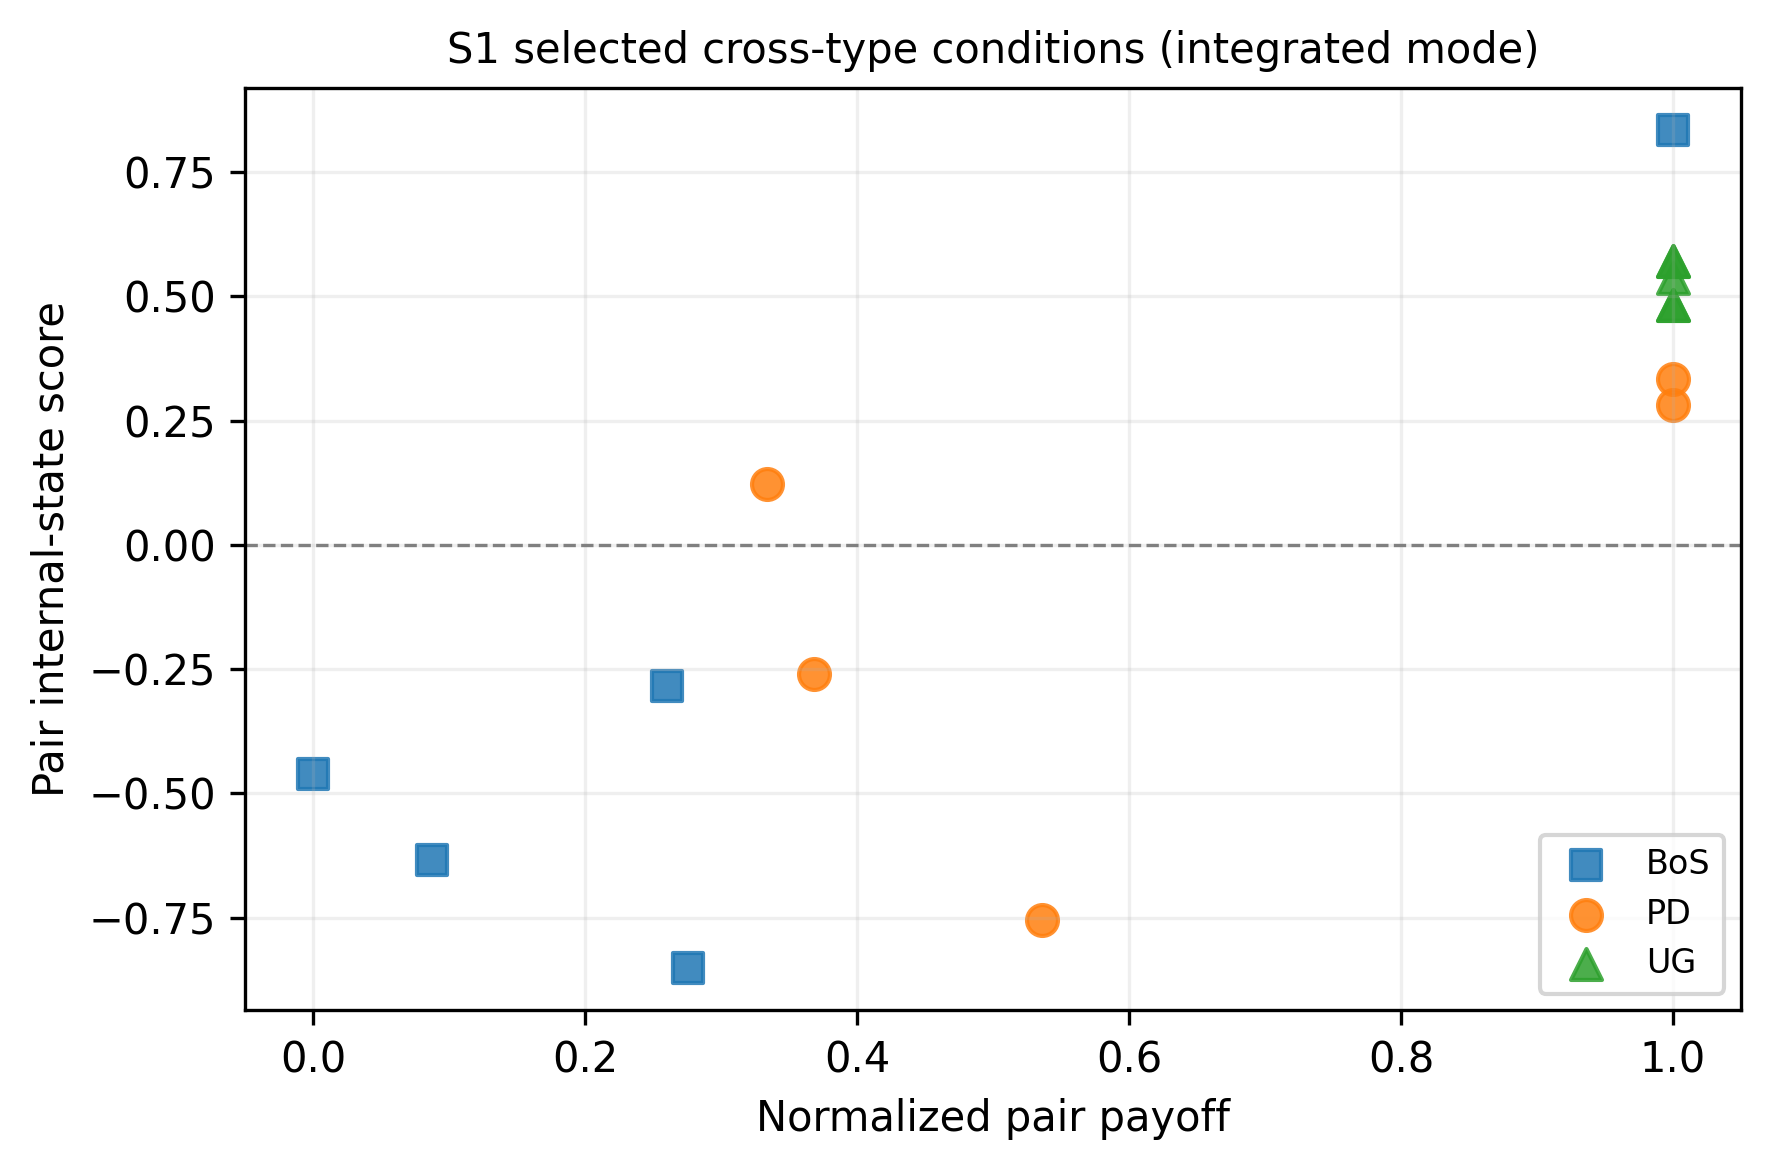
\includegraphics[width=.70\linewidth]{figures/fig_s1_selected_normalized_tradeoff.png}
\caption{S1 selected cross-type conditions in integrated mode. The plot uses normalized payoff to avoid mixing raw payoff scales across games.}
\label{fig:s1tradeoff}
\end{figure}

The results do not imply universal hybrid superiority. In PD, Hybrid--Hybrid and Fixed-TFT--Fixed-TFT both reach the cooperative optimum, whereas Hybrid--Rational and Emotional--Rational expose payoff/state asymmetries. In BoS, Fixed-TFT reaches stable coordination, but learned pairs remain weaker. In UG, several pairings achieve full acceptance, but this should be interpreted as a testbed outcome rather than human behavioral validity.

\subsection{S2: First-vs-Last-Third Trend Proxy}
S2 compares the first and last third of each episode. Table~\ref{tab:s2} reports the PD subset in integrated mode, where fixed-strategy semantics are cleanest. Figure~\ref{fig:s2pd} visualizes the same trend proxy. The word adaptation is used cautiously here: this is a within-episode behavioral shift, not a partner-switching experiment.

\begin{table}[t]
\centering
\caption{S2/PD first-vs-last-third proxy in integrated mode. Cooperation is reported as first-to-last; $\Delta$ payoff is agent 1 payoff change over the same thirds.}
\label{tab:s2}
\scriptsize
\begin{tabular}{llrrr}
\toprule
Agent & Fixed partner & Cooperation & $\Delta$ coop. & $\Delta$ payoff \\
\midrule
Emotional & Always-C & 1.000$\to$1.000 & 0.000 & 0.0 \\
Emotional & Always-D & 0.379$\to$0.424 & 0.045 & -3.0 \\
Emotional & TFT & 1.000$\to$1.000 & 0.000 & 0.0 \\
Hybrid & Always-C & 1.000$\to$1.000 & 0.000 & 0.0 \\
Hybrid & Always-D & 0.182$\to$0.030 & -0.152 & 10.0 \\
Hybrid & TFT & 1.000$\to$1.000 & 0.000 & 0.0 \\
Rational & Always-C & 0.000$\to$0.000 & 0.000 & 0.0 \\
Rational & Always-D & 0.000$\to$0.000 & 0.000 & 0.0 \\
Rational & TFT & 0.000$\to$0.000 & 0.000 & -4.0 \\
\bottomrule
\end{tabular}
\end{table}

\begin{figure}[t]
\centering
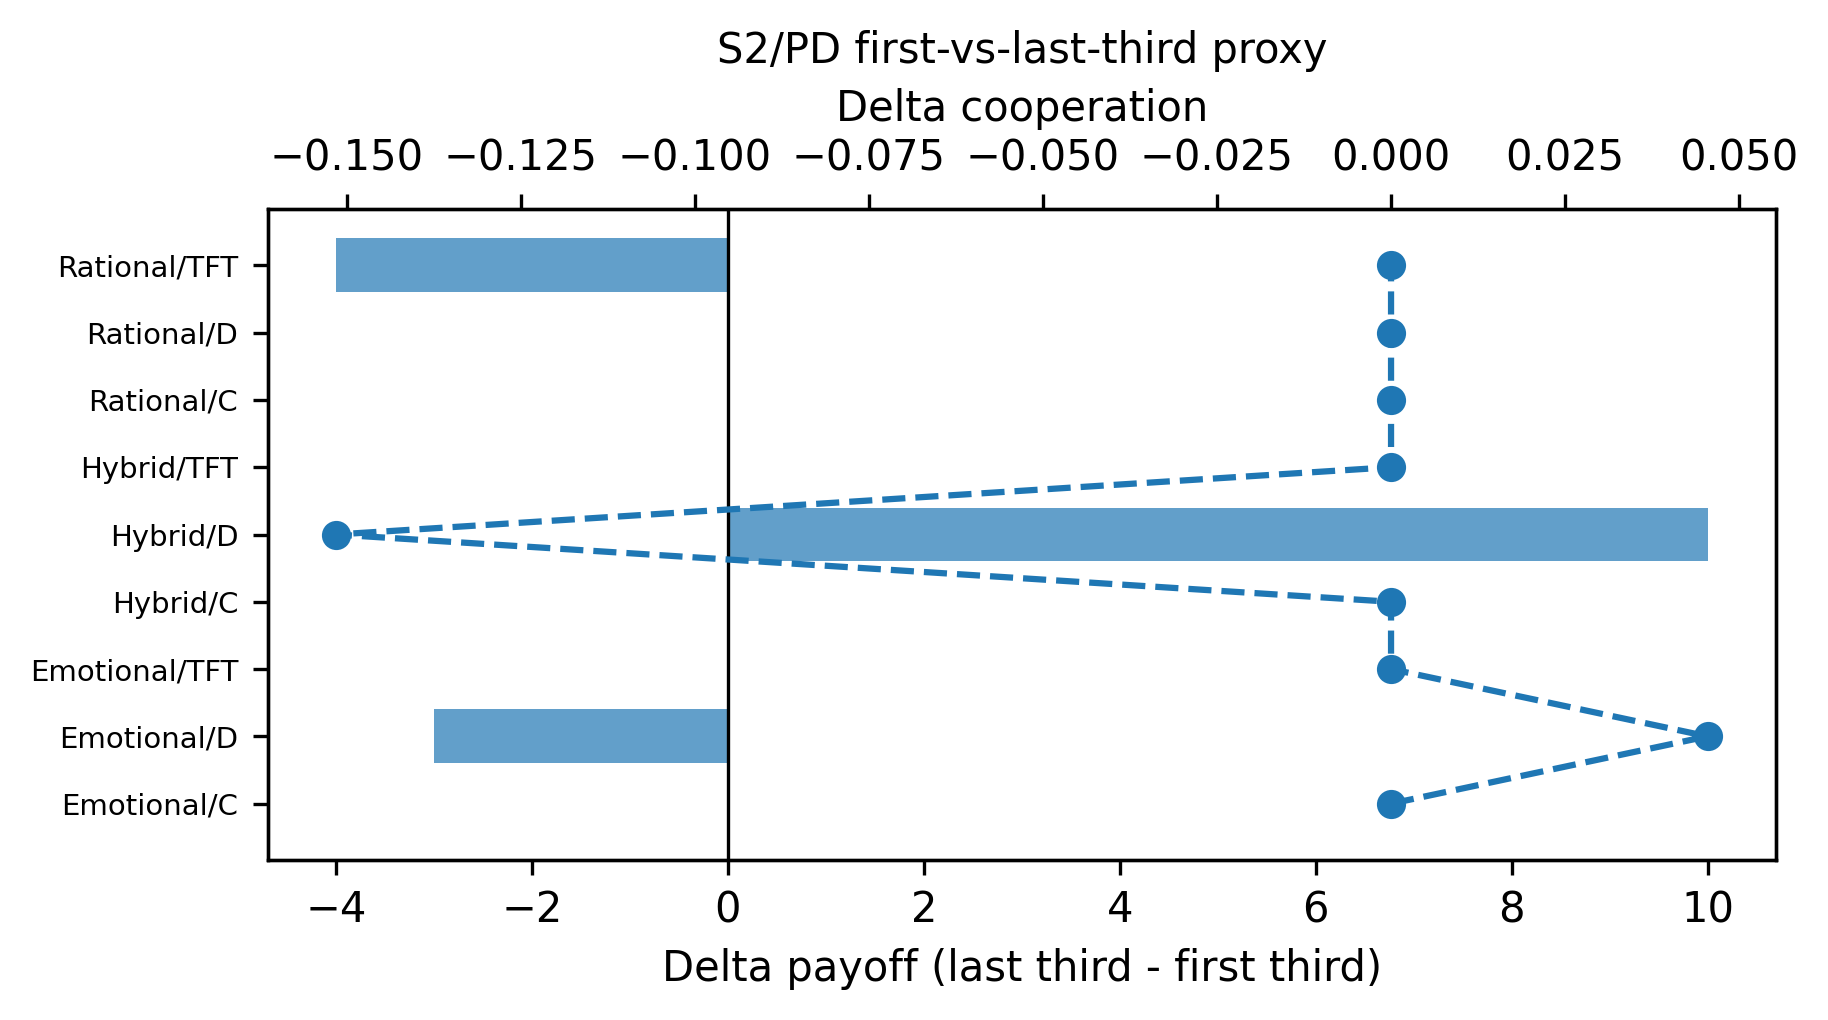
\includegraphics[width=.75\linewidth]{figures/fig_s2_pd_adaptation_clean.png}
\caption{S2/PD first-vs-last-third trend proxy. Bars show payoff change; points show cooperation change on a separate axis.}
\label{fig:s2pd}
\end{figure}

Hybrid and emotional agents maintain cooperation against always-cooperate and TFT partners. Against always-defect, the hybrid agent sharply reduces cooperation and gains payoff, whereas the emotional agent remains more cooperative. The rational agent defects throughout and therefore shows little first/last change. Thus RQ3 receives partial support only as a trend proxy.

\subsection{S3: Affective-Profile Sensitivity}
S3 is a profile/intensity sensitivity check, not a personality validation study. Table~\ref{tab:s3} shows that integrated-mode profile/intensity differences are moderate. Low intensity tends to have the highest mean state and normalized payoff among these aggregated PD cells, but the profile labels remain names for parameter settings, not psychological personality types.

\begin{table}[t]
\centering
\caption{S3 integrated-model profile/intensity aggregate in PD. Each row aggregates three fixed-partner conditions; payoff is normalized by the PD 200-round pair maximum.}
\label{tab:s3}
\scriptsize
\begin{tabular}{llrrr}
\toprule
Profile & Intensity & Norm. payoff & A1 state & A1 neg. share \\
\midrule
Neutral & high & 0.785 & 0.020 & 0.413 \\
Neutral & low & 0.797 & 0.085 & 0.333 \\
Neutral & neutral & 0.789 & 0.058 & 0.333 \\
Optimistic & high & 0.785 & 0.020 & 0.413 \\
Optimistic & low & 0.797 & 0.085 & 0.333 \\
Optimistic & neutral & 0.789 & 0.058 & 0.333 \\
Pessimistic & high & 0.789 & 0.014 & 0.413 \\
Pessimistic & low & 0.797 & 0.085 & 0.333 \\
Pessimistic & neutral & 0.789 & 0.058 & 0.333 \\
\bottomrule
\end{tabular}
\end{table}

\begin{figure}[t]
\centering
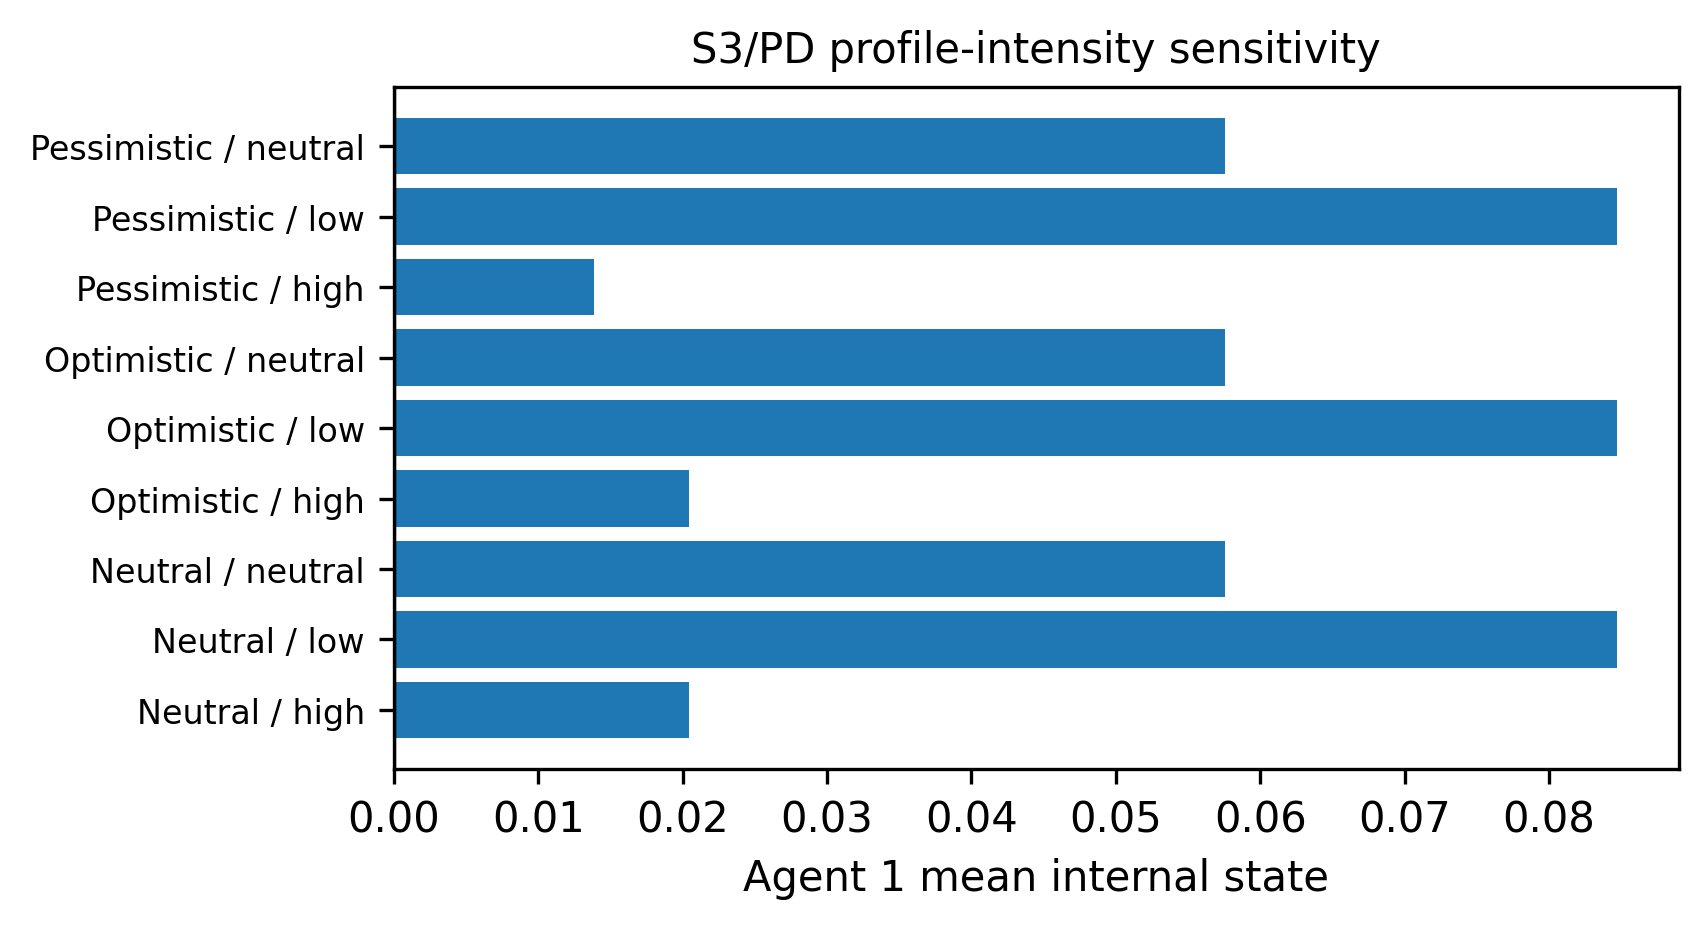
\includegraphics[width=.70\linewidth]{figures/fig_s3_profile_intensity_clean.png}
\caption{S3/PD profile-intensity sensitivity. The horizontal layout improves readability and emphasizes that differences are modest.}
\label{fig:s3}
\end{figure}

The near-repetition of some profile rows is itself informative: the current profile parameters have weaker effects than partner strategy and game structure. This motivates future sensitivity analysis over priorities, threshold parameters, and affective-intensity scaling.

\subsection{S4: Internal-State Diagnostics}
S4 tests selected diagnostic conditions. Table~\ref{tab:s4} shows that the integrated model no longer produces universal negative-state saturation. Favorable repeated regimes, such as PD Hybrid--Fixed-TFT and BoS Hybrid--Fixed-TFT, have both high normalized payoff and positive state. Poorly matched regimes remain negative, which is expected and useful for diagnosis.

\begin{table}[t]
\centering
\caption{S4 integrated-model internal-state diagnostics. Values are mean $\pm$ standard deviation over episodes.}
\label{tab:s4}
\scriptsize
\begin{tabular}{llcccc}
\toprule
Game & Pair & Norm. payoff & A1 state & A1 neg. & Metric \\
\midrule
PD & Hybrid vs Rational & 0.368 $\pm$ 0.000 & -0.389 $\pm$ 0.000 & 1.000 $\pm$ 0.000 & 0.0 \\
PD & Hybrid vs Fixed D & 0.368 $\pm$ 0.000 & -0.389 $\pm$ 0.000 & 1.000 $\pm$ 0.000 & 0.0 \\
PD & Hybrid vs Fixed TFT & 1.000 $\pm$ 0.000 & 0.281 $\pm$ 0.000 & 0.000 $\pm$ 0.000 & 1.0 \\
PD & Emotional vs Rational & 0.536 $\pm$ 0.000 & -1.043 $\pm$ 0.000 & 1.000 $\pm$ 0.000 & 0.0 \\
BoS & Hybrid vs Rational & 0.087 $\pm$ 0.160 & -0.760 $\pm$ 0.127 & 1.000 $\pm$ 0.000 & 0.0875 \\
BoS & Hybrid vs Fixed D & 0.087 $\pm$ 0.160 & -0.760 $\pm$ 0.127 & 1.000 $\pm$ 0.000 & 0.0875 \\
BoS & Hybrid vs Fixed TFT & 1.000 $\pm$ 0.000 & 0.742 $\pm$ 0.064 & 0.000 $\pm$ 0.000 & 1.0 \\
BoS & Emotional vs Rational & 0.260 $\pm$ 0.394 & -0.412 $\pm$ 0.538 & 0.761 $\pm$ 0.392 & 0.26 \\
UG & Hybrid vs Rational & 1.000 $\pm$ 0.000 & 0.537 $\pm$ 0.000 & 0.000 $\pm$ 0.000 & 1.0 / 5.0 \\
UG & Hybrid vs Fixed D & 0.000 $\pm$ 0.000 & -0.176 $\pm$ 0.000 & 1.000 $\pm$ 0.000 & 0.0 / 5.0 \\
UG & Hybrid vs Fixed TFT & 1.000 $\pm$ 0.000 & 0.537 $\pm$ 0.000 & 0.000 $\pm$ 0.000 & 1.0 / 5.0 \\
UG & Emotional vs Rational & 1.000 $\pm$ 0.000 & 0.537 $\pm$ 0.000 & 0.000 $\pm$ 0.000 & 1.0 / 5.0 \\
\bottomrule
\end{tabular}
\end{table}

\begin{figure}[t]
\centering
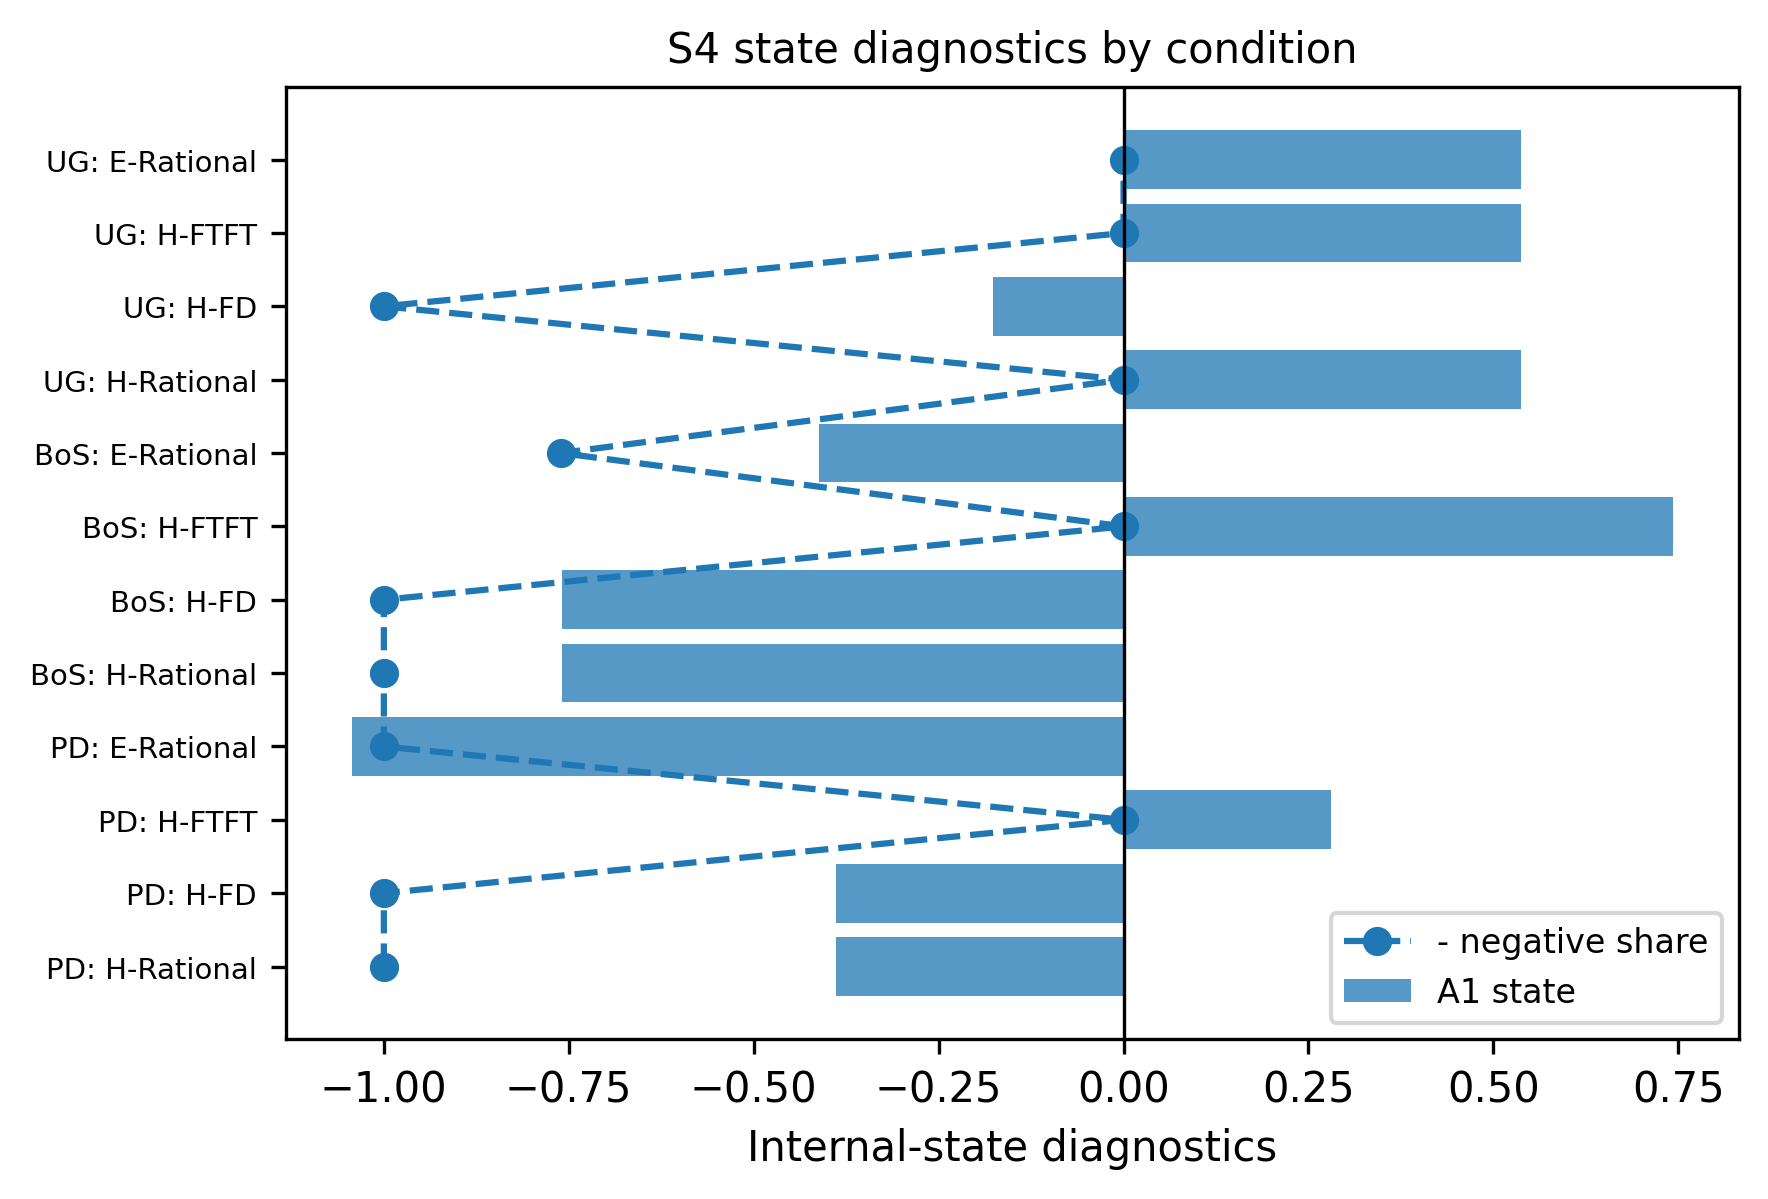
\includegraphics[width=.78\linewidth]{figures/fig_s4_diagnostics_clean.png}
\caption{S4 integrated-model state diagnostics. Bars show agent 1 mean state; points show negative-state share with sign reversed for visual comparison.}
\label{fig:s4}
\end{figure}

Figure~\ref{fig:s4} and Table~\ref{tab:s4} show that negative regimes are localized in specific game/partner settings. This answers RQ4 descriptively: state degradation reflects the interaction of value deltas, affective update, fatigue, game-specific semantics, and partner strategy. It is not merely a payoff failure, but it is also not an externally validated psychological diagnosis.

\section{Discussion}
The two-mode experiments clarify what the architecture contributes. The diagnostic-control mode preserves a conservative audit line, while the integrated mode tests whether external outcomes can become subjectively meaningful events before they shape later decisions. The main contribution is therefore a reproducible diagnostic implementation that makes this alignment inspectable and testable, not a proof that the resulting agents are human-like or generally superior.

RQ1 is supported at the architectural level: the same adapter/appraisal/state framework runs across PD, BoS, and UG and yields interpretable diagnostics without changing the overall architecture. RQ2 shows metric-dependent differences rather than dominance: normalized payoff, social metrics, and internal state can disagree. RQ3 receives only narrow support as a first-vs-last-third trend proxy under fixed partners. RQ4 is the clearest result: in the integrated model, negative-state regimes are no longer a uniform update artifact, but appear in specific game and partner regimes.

The central state score is internal to the model; improved state stability is therefore an interpretable diagnostic result, not external behavioral validation. This distinction is the main reason the paper is useful as part of a larger programme. It identifies the next tests that matter: ablations (no-adapter, no-mood, no-fatigue, shuffled-adapter, no-refocus), sensitivity analysis over state weights and update rates, stronger game-specific baselines, and human or observer validation of the adapter and state interpretations. The work is self-contained as an architecture and experimental study, but deliberately cumulative as a step toward explainable emotionally bounded-rational agents.

\section{Reproducibility and Artifacts}
The artifact bundle is available in the public GitHub repository \url{https://github.com/und3f1n3d5/EmBoRA}. The provided experiment package includes the LaTeX source, bibliography, generated tables and figures, architecture-aligned agent code, tests, experiment runner, configuration files, analyzed paper-run tables, selected figures, experiment report, validation summary, run inventory, and interpretation guardrails. The run manifests store seeds, strict/error policy, file hashes, and a code snapshot identifier; for the integrated S1 run, the snapshot identifier begins with \texttt{41f18ba89727}; the full hash is stored in the run manifests. The runs used here were executed as S1--S4 in two model modes with 20 episodes and 200 rounds, for example:
\begin{verbatim}
python experiment_runner.py --scenario S1 \
  --profile paper --games all \
  --model-mode integrated_model --strict --yes
\end{verbatim}
Figures and tables can be regenerated from saved outputs. Reported values are descriptive means and diagnostics; no significance tests are claimed.

\section{Scope, Safeguards, and Development Roadmap}
This article makes one specific claim: the proposed emotionally bounded-rational loop can be specified, implemented, audited, and stress-tested in repeated games. It does not ask the reader to accept human-behavioral validity or general performance advantages on faith. Those claims require another layer of evidence. The contribution here is the layer that must come first: a formalized game-to-values loop, two model modes, normalized game-sensitive metrics, and a traceable experimental package.

The next layer is explainability and causal diagnosis. The integrated model already makes value changes, appraisal, mood, fatigue, and state dynamics available for inspection, but the present paper does not yet claim that each decision is fully explained by a white-box rule. A planned white-box bounded-rational baseline will convert the same computational loop into per-turn traces: value update, appraisal, affective proposal, threshold check, rational override or refocus, and state update. This will make it possible to test whether the learned policies and the explicit rule-based mechanism fail or succeed for the same reasons.

The second layer is mechanism validation. The reported results show that internal-state dynamics carry information under the specified aggregation; they do not yet show which component is responsible for which part of the pattern. The planned ablation suite therefore targets the actual moving parts: no-adapter, shuffled-adapter, no-mood, no-fatigue, no-refocus, fixed-threshold, and alternative value-aggregation variants. Sensitivity checks over $\lambda$ weights, value-update rates, recovery coefficients, initial values, and profile parameters will test whether the observed state-stability patterns survive beyond a narrow configuration.

The third layer is comparison and external validation. The current baselines are adequate for the diagnostic purpose of this paper; broader claims require harder opponents and more specific alternatives: non-affective Q-learning/DQN, best-response or Nash-inspired policies, social-preference agents, UG threshold proposer/responder policies, and BoS alternation or coordination heuristics. Human or observer studies should then test whether the adapter dimensions--material payoff, fairness, relationship, and safety/no-regret--match plausible social interpretations of the same outcomes. That is the validation path; presenting the current model as human-like or universally superior would be premature.

\section{Conclusion}
We presented an implementation-aware specification of emotionally bounded-rational agents for repeated games and evaluated it with architecture-aligned paper-profile experiments. The architecture separates external outcomes from internal value interpretation and makes payoff--state divergence inspectable. Under the specified internal-state aggregation, the integrated mode yields higher state scores and lower negative-state share than the diagnostic-control mode across the tested scenarios, while still exposing exploitation, coordination failure, and stress-test artifacts.

The article is self-contained as a computational specification and diagnostic state-stability study, while also serving as the foundation for the next stages of the research programme. Its role is to make emotionally bounded-rational mechanisms observable and reproducible without claiming human-subject validation, psychometric measurement validity, statistical superiority, or SOTA MARL performance. The immediate continuation is an explainability and validation layer: per-turn causal traces, ablations of mood, fatigue, refocus, and value dimensions, stronger game-specific baselines, sensitivity analysis, and human or observer evaluation of whether the adapter and internal-state diagnostics capture plausible social interpretations.

\subsubsection*{Acknowledgments.}
The authors thank colleagues and reviewers whose comments helped improve the architecture, experimental protocol, and positioning of the work. Generative AI tools were used for language polishing, structural revision support, code validation and analysis, and artifact organization; the authors remain responsible for all claims, experiments, and final text.

\bibliographystyle{splncs04}
\bibliography{eumas2026_references_camera_ready}

\end{document}
